\documentclass[Afour,sageh,times]{sagej}
\usepackage[utf8]{inputenc}
\usepackage[USenglish]{babel}
\usepackage{booktabs}
\usepackage{setspace}
\usepackage{csquotes}
\usepackage{url}
\usepackage{moreverb}
\usepackage[colorlinks,bookmarksopen,bookmarksnumbered,citecolor=red,urlcolor=red]{hyperref}
\newcommand\BibTeX{{\rmfamily B\kern-.05em \textsc{i\kern-.025em b}\kern-.08em T\kern-.1667em\lower.7ex\hbox{E}\kern-.125emX}}


\def\volumeyear{\the\year}




\begin{document}

\runninghead{Author Redacted}
\title{The Importance of Being Nonplanar: Street Network Representation in Urban Form Studies}
\author{Author Redacted \affilnum{1}}
\affiliation{\affilnum{1}Affiliation redacted}
\corrauth{Author Redacted, Address Redacted}
\email{Email Redacted}


\begin{abstract}

\end{abstract}

\keywords{street network, GIS, urban form, transportation, urban design}

\maketitle

\section{Introduction}




\section{Background}

Why it's appealing. Planarity allows for easy polygonal spatial analysis \citep{fohl_non-planar_1996}. In mathematics, there is an exact bijection between planar graphs and trees, and classifying planar graphs presents a trivial computational problem \citep{louf_typology_2014}. Planar graphs offer computational simplicity and tractability. But \citet{masucci_random_2009} and \citet{masucci_limited_2013} argue that planar graphs have also presented a compelling research domain for urban scholars and geographers as they were understudied until recently because they appear topologically and geometrically trivial and the planarity constraint did not lend itself to certain popular graph-theoretic analyses. By contrast, \citet[p.~3]{barthelemy_spatial_2011} argue that \enquote{planar spatial networks are the most important and most studies have focused on these examples}. As \citet[p.~1]{viana_simplicity_2013} put it, \enquote{there is still a lack of global, high-level metrics allowing to characterize their structure and geometrical patterns.}

Street networks, however, are frequently nonplanar in reality: they tend to have some overpasses or underpasses that result in the failure of formal proofs of their planarity, such as the \citet{kuratowski_sur_1930} theorem or the \cite{hopcroft_efficient_1974} algorithm \citep{gastner_spatial_2006}. As \citet[p.~7]{levinson_network_2012} points out, \enquote{Real networks are neither perfect, nor planar, nor grids, though they may approximate them.} \enquote{Quite often the transportation network has overpasses and underpasses that require a non-planar network representation} \citet[p.~199]{jiang_object-oriented_2010}. \enquote{A planar graph is one which can be drawn in two dimensions with no edges intersecting except at vertices on which they are both incident. For many infrastructure networks, this is approximately true, although bridges and tunnels in ground-transport networks are an obvious (but generally minor) exception.} \citet[p.~1258]{fischer_spatial_2014}.

Twenty years ago, \citep[p.~18]{fohl_non-planar_1996} claimed, \enquote{The most commonly used data model for transportation networks is the fully intersected, planar data model} and called for a nonplanar model to better represent truly nonplanar spatial networks.

\enquote{The planar network data model has received widespread acceptance and use. Despite its popularity, the
model has limitations for some areas of transportation analysis, especially where complex network structures
are involved. One major problem is caused by the planar embedding requirement... intersections at grade cannot be distinguished from intersections with an overpass or underpass that do not cross at grade.} \citep[p.~395]{fischer_gis_2004}

\citet[p.~6]{kwan_review_1996} \enquote{the difficulty in accurately representing overpasses or underpasses may lead to problems when running various routing algorithms (e.g. recommending that a traveler make a left-turn at an intersection that proves to be an overpass!)}.

\begin{table*}[htbp]
\centering
\caption{Recent statements in the urban studies and urban physics literatures regarding the representation of street networks as planar graphs.}
\label{table:planar_quotes}
\begin{tabular}{ | p{0.95\textwidth} | }
\toprule

\enquote{In a planar graph, no links intersect, except by nodes. This feature represents a transportation network well.} \citep[p.~6]{dill_measuring_2004} \\ \hline

\enquote{Street networks are planar graphs composed of junctions and street segments...} \citep[p.~18]{batty_network_2005} \\ \hline

\enquote{The number of long-range connections and the number of edges that can be connected to a single node are limited by the spatial embedding. This is particularly evident in planar networks e.g., those networks forming vertices whenever two edges cross, as urban streets or ant networks of galleries...} \citep[p.~1]{crucitti_centrality_2006} \\ \hline

\enquote{Any of these street networks (SNS) can be described by an embedded planar graph... Street networks are planar graphs and such planarity strongly constrains their heterogeneity...} \citep[pp.~514~\&~521]{buhl_topological_2006} \\ \hline

\enquote{Planar graphs are those graphs forming vertices whenever two edges cross, whereas nonplanar graphs can have edge crossings that do not form vertices. The graphs representing urban street patterns are, by construction, planar...} \citep[p.~3]{cardillo_structural_2006} \\ \hline

\enquote{The connection and arrangement of a road network is usually abstracted in network analysis as a directed planar graph...} \citep[p.~340]{xie_measuring_2007} \\ \hline

\enquote{Urban street patterns form planar networks... The simplest description of the street network consists of a graph whose links represent roads and whose vertices represent road intersections and end points. For these graphs, links intersect essentially only at vertices and are thus planar.} \citep[p.~1]{barthelemy_modeling_2008} \\ \hline

\enquote{Urban street networks as spatial networks are embedded in planar space, which give many constraints.} \citep[p.~1]{hu_topological_2008} \\ \hline

\enquote{...a street network is a strange network when compared to other social or biological networks in the sense that it is embedded in the Euclidian space and the edges do not cross each other. In graph theory, such a network is called a planar graph.} \citep[p.~259]{masucci_random_2009} \\ \hline

\enquote{...street networks are embedded in space and are planar in nature...} \citep[p.~114]{porta_networks_2010} \\ \hline

\enquote{Roads, rail, and other transportation networks are spatial and to a good accuracy planar networks. For many applications, planar spatial networks are the most important...} \citep[p.~3]{barthelemy_spatial_2011} \\ \hline

\enquote{...urban road systems can be (in good approximation) considered as planar networks, i.e., links cannot \enquote{cross} each other without forming a physical intersection (node) as long as there are no tunnels or bridges... The meaningful definition of link angles requires the presence of a planar network, which is assumed to be the case in urban road systems.} \citep[pp.~563~\&~567]{chan_urban_2011} \\ \hline

\enquote{Road networks are planar graphs consisting of a series of land cells surrounded by street segments.} \citep[p.~3]{strano_elementary_2012} \\ \hline

\enquote{Planar graphs are basic tools for understanding transportation systems embedded in two-dimensional space, in particular urban street networks... As these graphs are embedded in a two-dimensional surface, the
planarity criteria requires that the links do not cross each other.} \citep[p.~1]{masucci_limited_2013} \\ \hline

\enquote{...street networks are essentially planar; in the absence of tunnels and bridges, the streets (the links) cannot cross without generating an intersection or a junction, that is, a node.} \citep[p.~1]{gudmundsson_entropy_2013}. \\ \hline

\enquote{Networks of street patterns belong to a particular class of graphs called planar graphs, that is, graphs whose links cross only at nodes.} \citep[p.~1074]{strano_urban_2013} \\ \hline

\enquote{In city science, planar networks are extensively used to represent, to a good approximation, various infrastructure networks... in particular, transportation networks and more recently streets patterns...} \citep[p.~1]{viana_simplicity_2013} \\ \hline

\enquote{...finding a typology of street patterns essentially amounts to classifying planar graphs...} \citep[p.~2]{louf_typology_2014} \\ \hline

\enquote{...we are dealing with spatial graphs, which tend to be planar...} \citep[p.~2191]{zhong_detecting_2014} \\ \hline

\enquote{Urban transport systems as networks can be represented as planar graphs...} \citep[p.~2]{wang_resilience_2015} \\ \hline

\enquote{In graph theory, a spatial street network is a type of planar graph embedded in Euclidean space.} \citep[p.~168]{law_defining_2017} \\ \hline

\bottomrule
\end{tabular}
\end{table*}







\section{Methods}

Cardillo et al use one square mile of different world cities.

We formally test for planarity using the method described by \citet{boyer_subgraph_2012}.








\section{Results}

\begin{figure*}[htbp]
    \center
    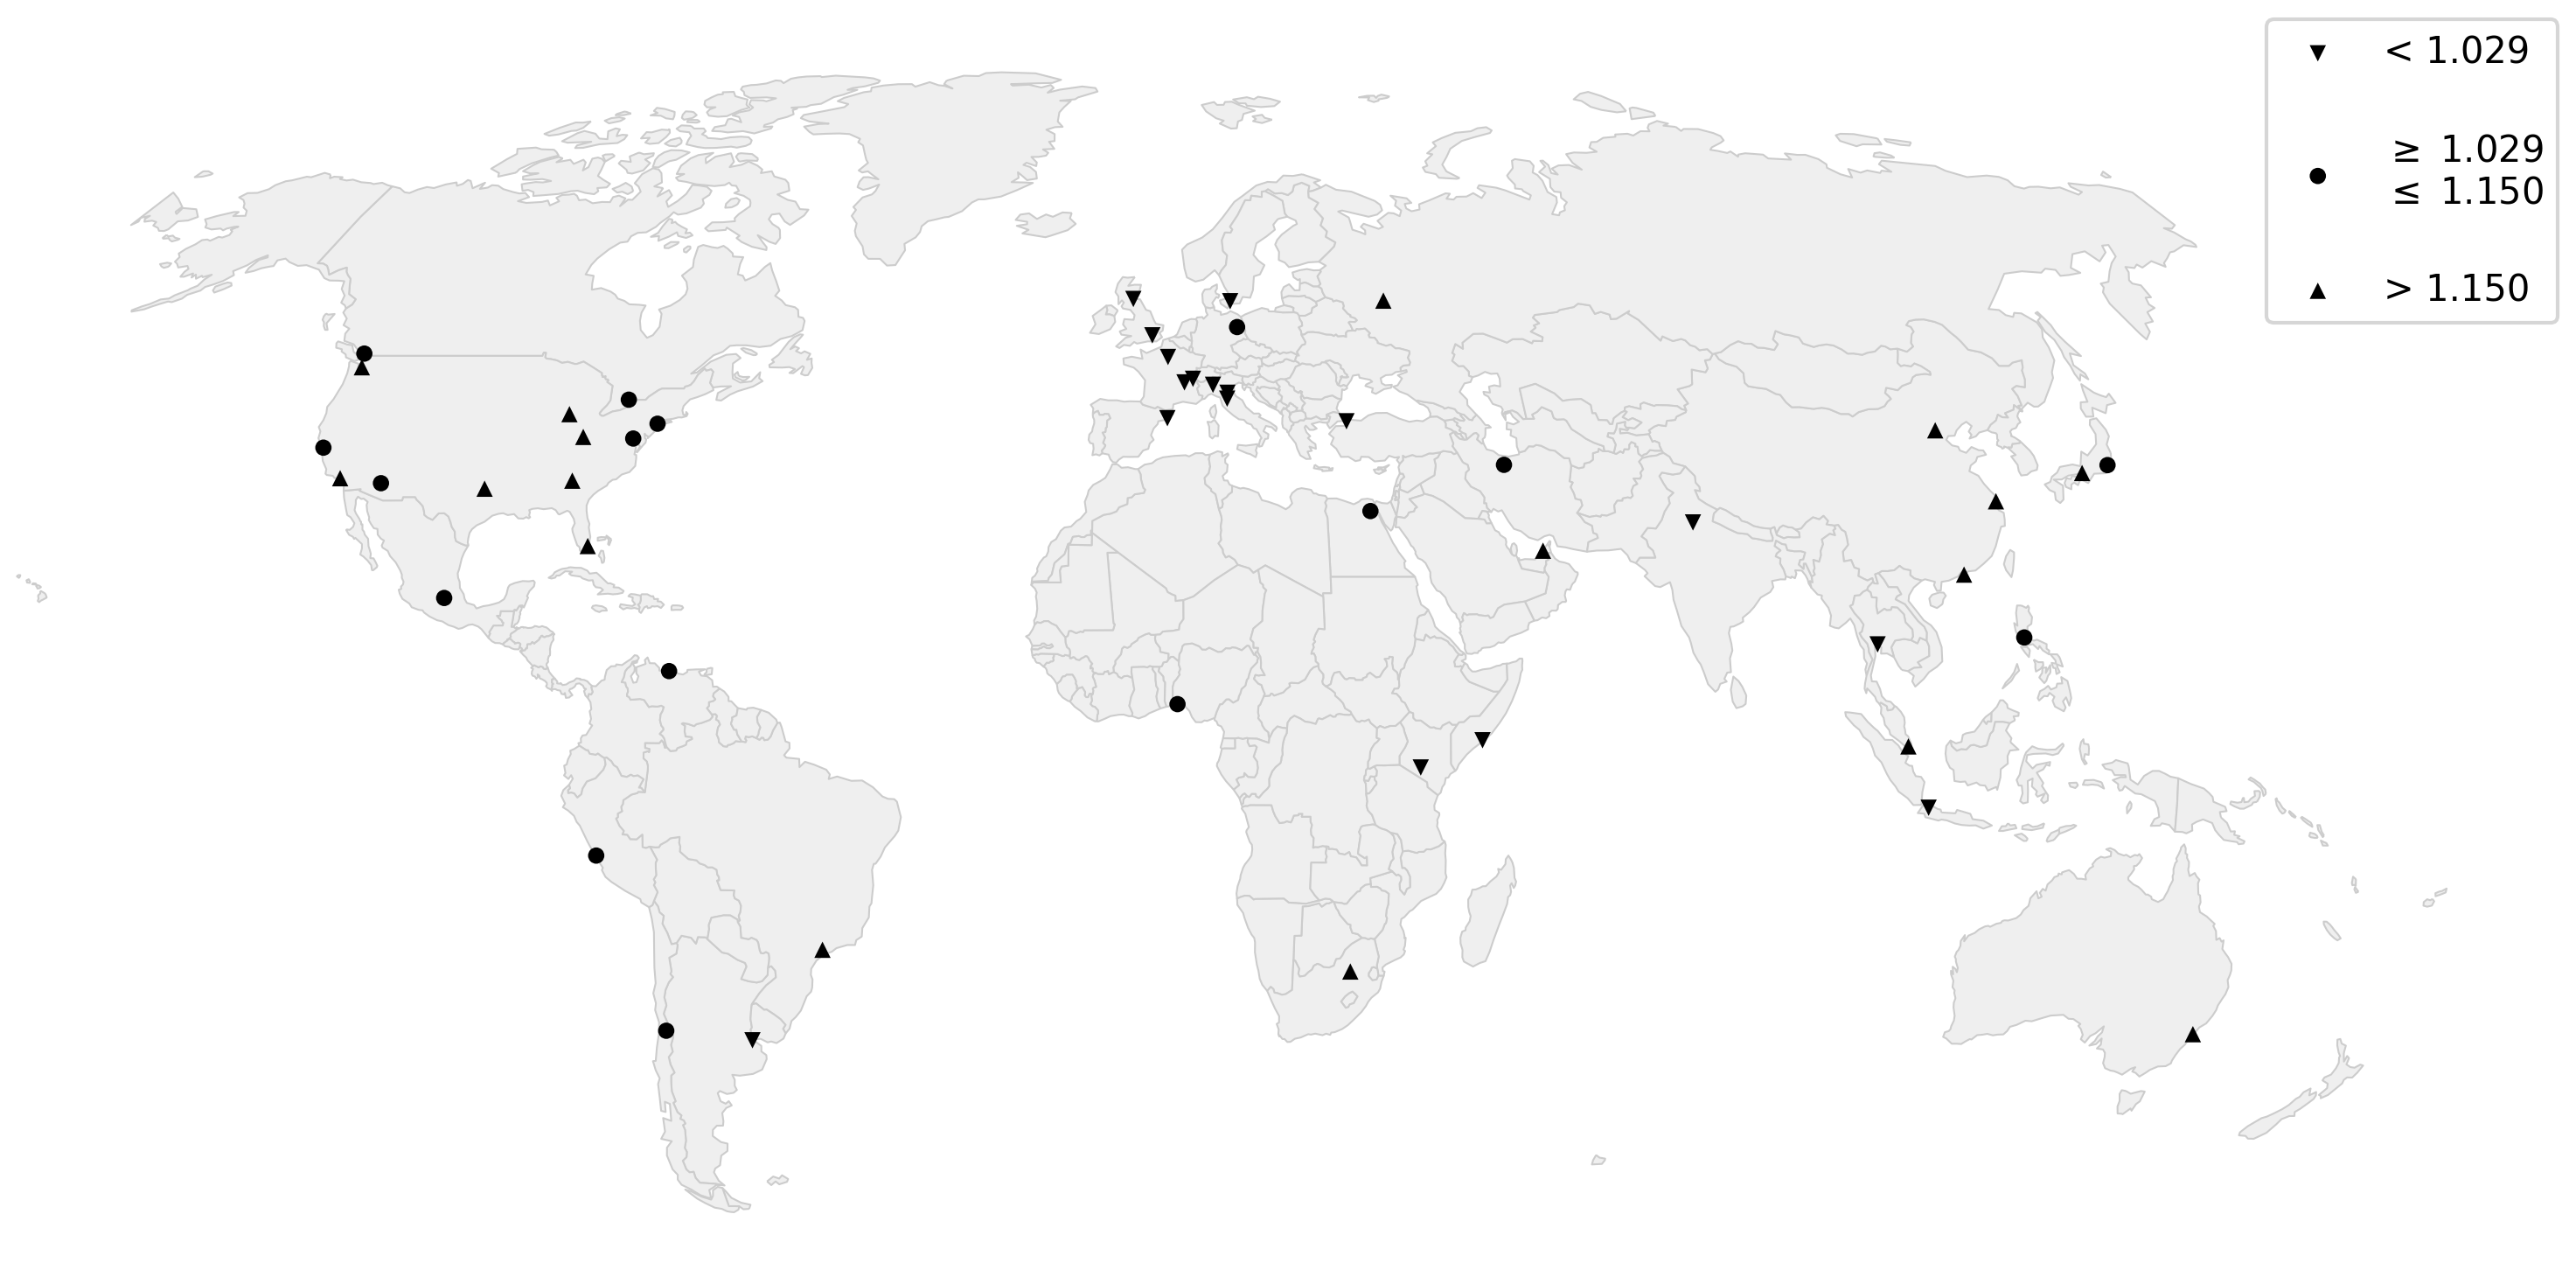
\includegraphics[width=\textwidth]{world_map_bw.png}
    \caption{Map of world cities in Table \ref{tab:cities} grouped by OPN score tertiles.}
    \label{fig:world_map_opn}
\end{figure*}


\begin{table*}[htbp]
\centering
\caption{Across many cities.}
\label{tab:cities}
\begin{tabular}{ l l l r r r l r r r }
\toprule
             &               & \multicolumn{4}{|c|}{Drive}         & \multicolumn{4}{c}{Walk}            \\
\midrule
Country      & City          &  Planar  &  OPN   &  ONC   &  ELR   &  Planar  &  OPN   &  ONC   &  ELR   \\
\midrule
Argentina    & Buenos Aires  &      Yes &  1.000 &  1.052 &  1.000 &       No &  1.057 &  2.241 &  0.947 \\
Australia    & Sydney        &       No &  1.350 &  1.172 &  0.749 &       No &  1.100 &  1.619 &  0.901 \\
Brazil       & Sao Paulo     &       No &  1.264 &  1.146 &  0.790 &       No &  1.174 &  1.404 &  0.831 \\
Canada       & Toronto       &      Yes &  1.075 &  1.054 &  0.958 &       No &  1.165 &  4.763 &  0.848 \\
             & Vancouver     &       No &  1.077 &  1.064 &  0.948 &       No &  1.077 &  1.538 &  0.926 \\
Chile        & Santiago      &       No &  1.143 &  1.074 &  0.887 &       No &  1.028 &  1.261 &  0.971 \\
China        & Beijing       &       No &  1.223 &  1.754 &  0.872 &       No &  1.188 &  1.743 &  0.848 \\
             & Hong Kong     &       No &  1.183 &  1.317 &  0.835 &       No &  1.190 &  1.837 &  0.818 \\
             & Shanghai      &       No &  1.466 &  1.615 &  0.717 &       No &  1.494 &  1.751 &  0.659 \\
Denmark      & Copenhagen    &      Yes &  1.008 &  1.175 &  0.988 &       No &  1.009 &  1.703 &  0.987 \\
Egypt        & Cairo         &       No &  1.111 &  1.110 &  0.916 &       No &  1.090 &  1.233 &  0.906 \\
France       & Lyon          &       No &  1.009 &  1.225 &  0.989 &       No &  1.042 &  1.647 &  0.957 \\
             & Paris         &       No &  1.012 &  1.163 &  0.993 &       No &  1.087 &  1.632 &  0.917 \\
Germany      & Berlin        &       No &  1.065 &  1.267 &  0.950 &       No &  1.061 &  2.183 &  0.936 \\
India        & Delhi         &      Yes &  1.000 &  1.462 &  1.000 &      Yes &  1.007 &  1.465 &  0.992 \\
Indonesia    & Jakarta       &      Yes &  1.017 &  1.218 &  0.986 &       No &  1.040 &  1.374 &  0.960 \\
Iran         & Tehran        &       No &  1.040 &  1.350 &  0.973 &       No &  1.045 &  1.478 &  0.956 \\
Italy        & Bologna       &      Yes &  1.000 &  1.218 &  1.000 &      Yes &  1.004 &  2.267 &  0.996 \\
             & Florence      &      Yes &  1.000 &  1.212 &  1.000 &       No &  1.021 &  1.464 &  0.978 \\
             & Milan         &      Yes &  1.000 &  1.259 &  1.000 &       No &  1.142 &  2.399 &  0.860 \\
Japan        & Osaka         &       No &  1.152 &  1.215 &  0.871 &       No &  1.051 &  2.475 &  0.949 \\
             & Tokyo         &       No &  1.078 &  1.333 &  0.923 &       No &  1.084 &  1.723 &  0.912 \\
Kenya        & Nairobi       &       No &  1.027 &  1.372 &  0.974 &       No &  1.054 &  1.382 &  0.943 \\
Mexico       & Mexico City   &       No &  1.064 &  1.249 &  0.952 &       No &  1.096 &  1.386 &  0.917 \\
Nigeria      & Lagos         &       No &  1.050 &  1.085 &  0.967 &       No &  1.012 &  1.076 &  0.987 \\
Peru         & Lima          &       No &  1.065 &  1.344 &  0.941 &       No &  1.072 &  1.747 &  0.931 \\
Philippines  & Manila        &       No &  1.057 &  1.192 &  0.953 &       No &  1.104 &  1.392 &  0.895 \\
Russia       & Moscow        &       No &  1.743 &  1.186 &  0.680 &       No &  1.168 &  1.875 &  0.858 \\
Singapore    & Singapore     &       No &  1.152 &  1.375 &  0.874 &       No &  1.113 &  1.907 &  0.890 \\
Somalia      & Mogadishu     &      Yes &  1.000 &  1.044 &  1.000 &      Yes &  1.000 &  1.047 &  1.000 \\
South Africa & Johannesburg  &       No &  1.176 &  1.057 &  0.883 &       No &  1.003 &  1.056 &  0.997 \\
Spain        & Barcelona     &      Yes &  1.000 &  1.265 &  1.000 &       No &  1.106 &  1.923 &  0.900 \\
Switzerland  & Geneva        &       No &  1.015 &  1.249 &  0.982 &       No &  1.207 &  2.613 &  0.813 \\
Thailand     & Bangkok       &       No &  1.012 &  1.258 &  0.988 &       No &  1.007 &  1.349 &  0.989 \\
Turkey       & Istanbul      &       No &  1.026 &  1.222 &  0.982 &       No &  1.020 &  1.490 &  0.978 \\
UAE          & Dubai         &       No &  1.460 &  1.303 &  0.722 &       No &  1.163 &  1.457 &  0.850 \\
UK           & Edinburgh     &       No &  1.027 &  1.333 &  0.968 &       No &  1.012 &  2.231 &  0.988 \\
             & London        &       No &  1.022 &  1.276 &  0.981 &       No &  1.157 &  2.734 &  0.847 \\
USA          & Atlanta       &       No &  1.359 &  1.042 &  0.777 &       No &  1.355 &  2.030 &  0.724 \\
             & Chicago       &       No &  1.289 &  1.414 &  0.814 &       No &  1.240 &  2.671 &  0.804 \\
             & Cincinnati    &       No &  1.370 &  1.141 &  0.757 &       No &  1.074 &  1.482 &  0.927 \\
             & Dallas        &       No &  1.672 &  1.311 &  0.650 &      Yes &  1.039 &  1.819 &  0.959 \\
             & Los Angeles   &       No &  1.717 &  1.111 &  0.635 &       No &  1.261 &  2.089 &  0.799 \\
             & Miami         &       No &  1.545 &  1.189 &  0.662 &       No &  1.037 &  1.617 &  0.961 \\
             & New York      &       No &  1.135 &  1.144 &  0.901 &       No &  1.062 &  2.026 &  0.941 \\
             & Phoenix       &       No &  1.047 &  1.206 &  0.962 &       No &  1.022 &  2.710 &  0.977 \\
             & San Francisco &       No &  1.070 &  1.093 &  0.941 &       No &  1.055 &  1.706 &  0.944 \\
             & Seattle       &       No &  1.367 &  1.047 &  0.779 &       No &  1.072 &  3.122 &  0.926 \\
             & Washington DC &       No &  1.055 &  1.351 &  0.956 &       No &  1.034 &  3.169 &  0.967 \\
Venezuela    & Caracas       &       No &  1.049 &  1.230 &  0.957 &      Yes &  1.000 &  1.254 &  1.000 \\
\bottomrule
\end{tabular}
\end{table*}




\begin{figure*}[htbp]
    \center
    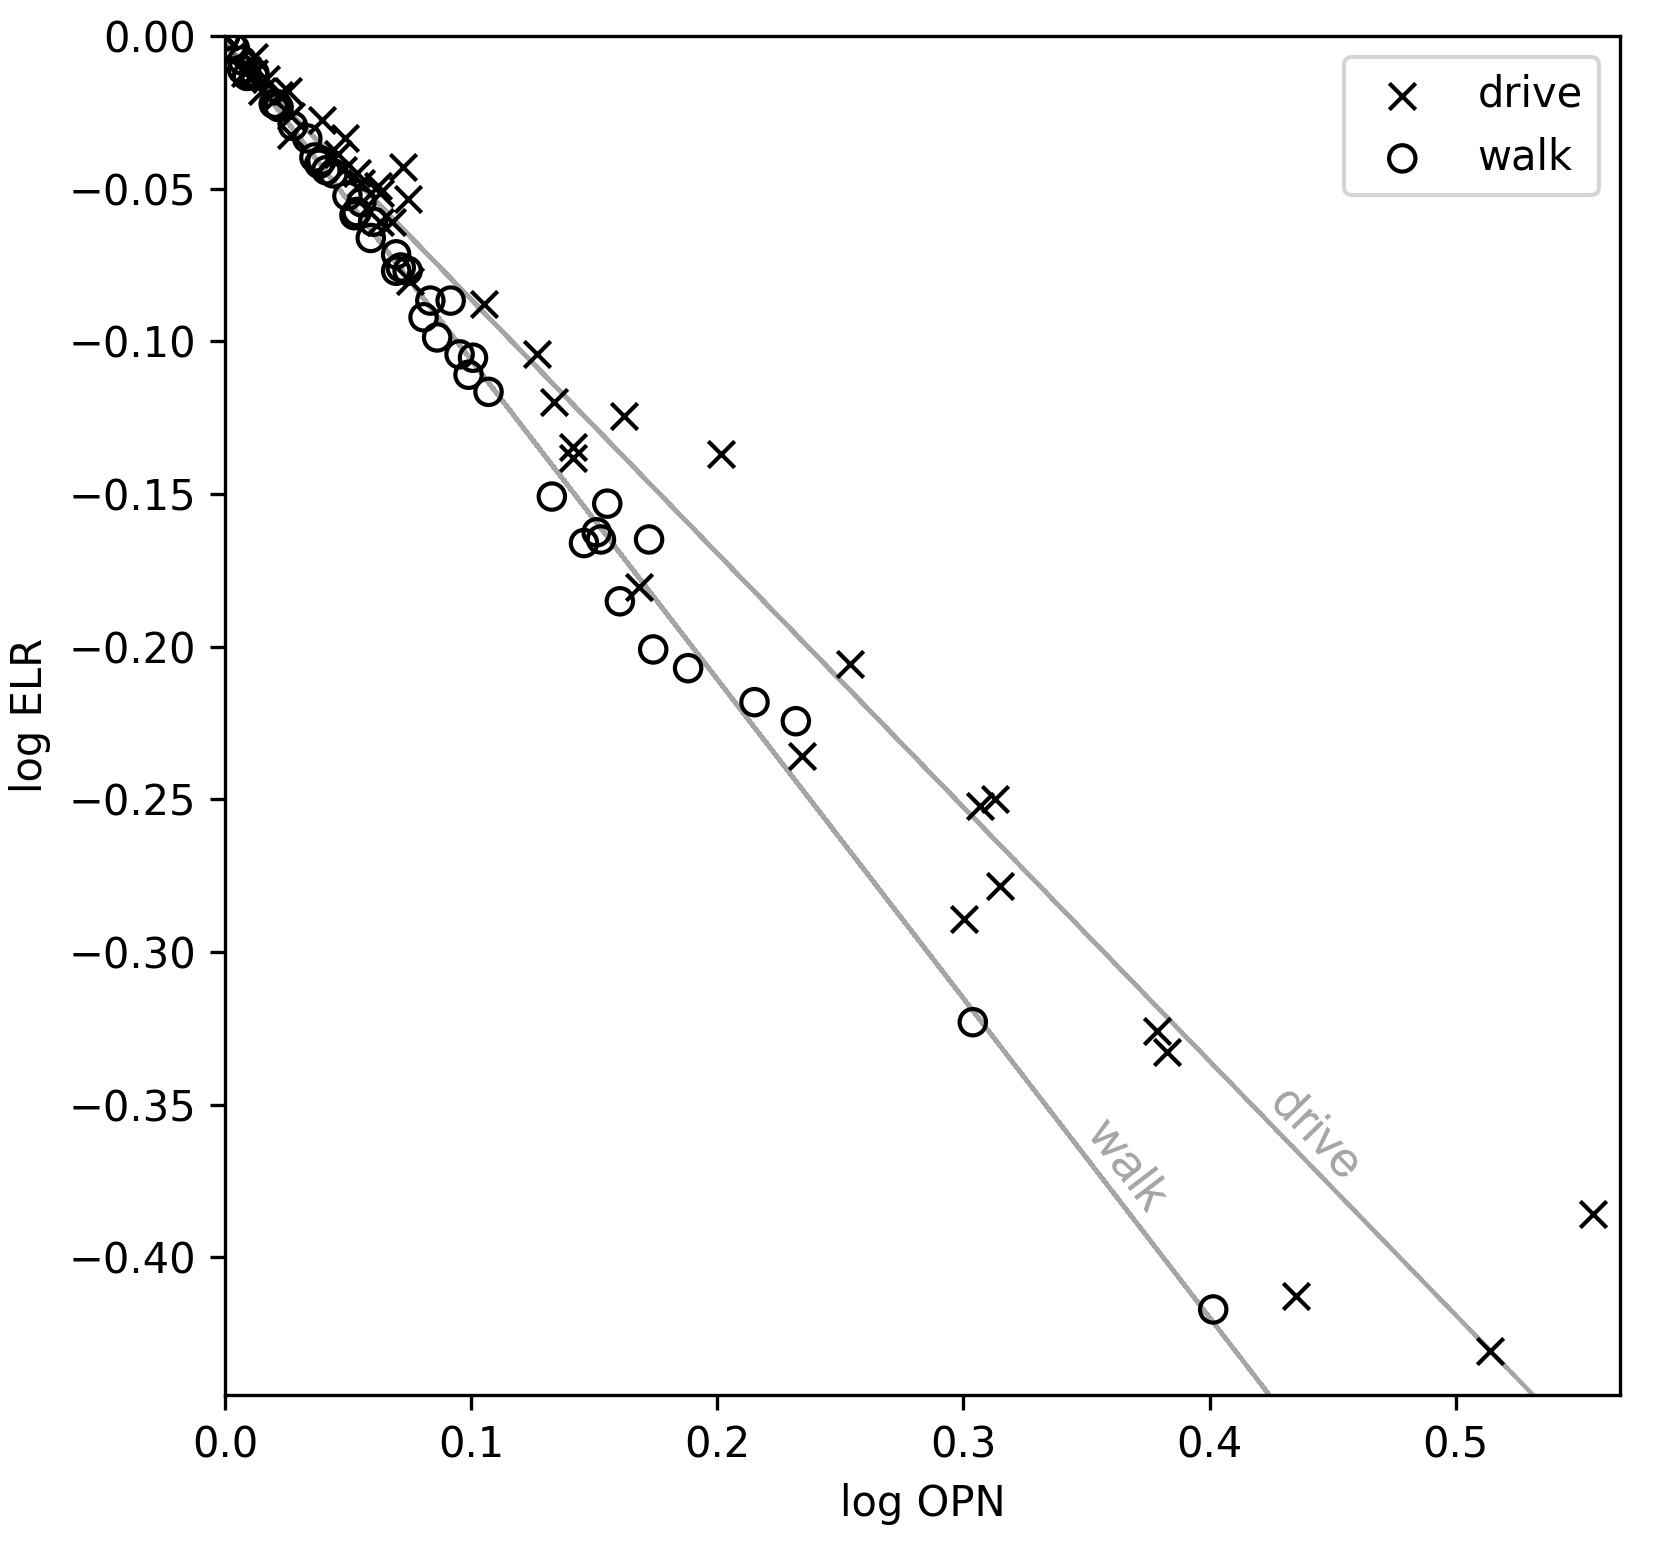
\includegraphics[width=0.5\textwidth]{regression_split.png}
    \caption{Log-log plot of ELR vs OPN with simple regression lines: drive $r^2=0.98$ and walk $r^2=0.99$.}
    \label{fig:regression_elr_opn}
\end{figure*}





\begin{table*}[htbp]
\centering
\caption{100 random square mile sample runs across one city, Oakland CA.}
\label{tab:samples_city}
\begin{tabular}{ l r r r r }
\toprule
         &  OPN   &  ONC   &  OPC   &  ELR   \\
\midrule
mean &                       1.091 &                        1.149 &                     1.256 &              0.947 \\
$\sigma$  &                       0.154 &                        0.120 &                     0.226 &              0.082 \\
min  &                       1.000 &                        1.000 &                     1.000 &              0.637 \\
max  &                       1.759 &                        1.833 &                     2.011 &              1.000 \\
\bottomrule
\end{tabular}
\end{table*}


\section{Discussion}

The point: street networks are regularly nonplanar in the formal sense. They are embedded in three dimensions and have a z-value along with their x and y. Because they are mostly planar, typically with only a few overpasses or underpasses, they could often be described accurately as \emph{quasi-planar}. However, claiming that urban street networks broadly are planar misrepresents them in several ways.

1. Forces false nodes where grade-separated edges cross.

2. Accordingly, underestimates average edge length (a proxy for street segment lengths and block sizes)

3. Misrepresents connectivity for routing, accessibility analysis, and other connectivity studies

\bibliographystyle{apa}
\bibliography{references}

\end{document}
